% !TEX root = QlockToo.tex

\section{Konstruktion und Produktion}
\label{sec:KonstruktionFertigung}

\begin{multicols}{2}
Um Kosten zu sparen wird die ClockToo als eine Kombination aus Kaufteilen und eigener Produktion ausgeführt. Ziel ist eine möglichst getreue Nachbildung der Original CLOCKTWO® der Biegert~\&~Funk Manufacture GmbH \& Co. KG. 

\textbf{Das Uhrgehäuse}

Die Basis für das Uhrengehäuse bildet der IKEA-Bilderrahmen RIBBA in schwarz. Die Bilddarstellungsmaße von 50 x 50 cm eigenen sich gut, um die Buchstabenmatrix zur Geltung zu bringen. In dem besonders tiefen Rahmen,  Tiefe~=~4,5~cm, kann die komplette LED-Matrix inklusive der Elektronik untergebracht werden. Lediglich zum Hinausführen des Stromkabels und zur Anbringung der Taster muss der Rahmen leicht modifiziert werden. 

{
\centering 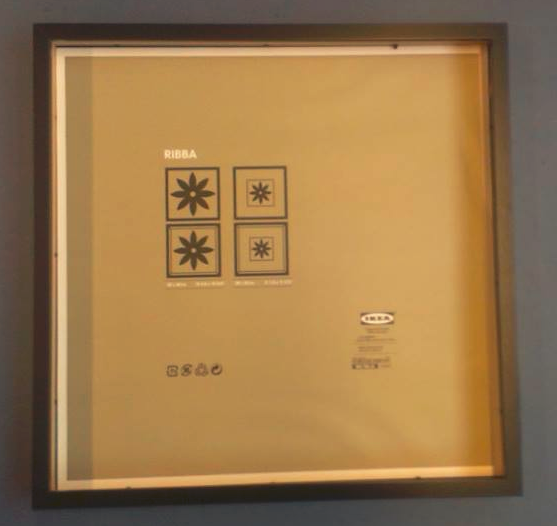
\includegraphics[width=0.85\columnwidth]{Abbildungen/Konstruktion/Ribba} %Bilderrahmen

}
\textbf{Buchstabenfolie}


Zur Darstellung der Buchstaben wird eine schwarze Folie mit der negativen Buchstabenmatrix auf eine Plexiglasscheibe geklebt. Die Anordnung der Buchstaben entspricht der Anordnung der Original CLOCKTWO®. 

{
\centering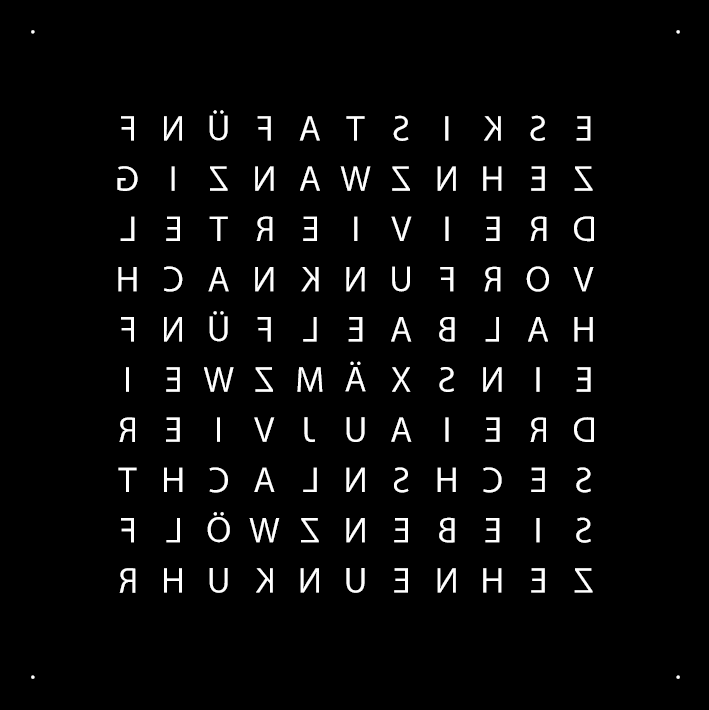
\includegraphics[width=0.85\columnwidth]{Abbildungen/Konstruktion/Buchstaben}

}
Mit dieser Buchstabenmatrix ist die Uhr auf eine deutsche Anzeige festgelegt. Die Original CLOCKTWO® CLASSIC beherscht zwölf Sprachen. Durch Austauschen des Frontcovers kann die gewünschte Sprache eingestellt werden. 

\textbf{LED-Matrix}

Die LED-Matrix wird aus einer quadratischen Spanplatte gefertigt. Abbildung~\ref{fig:Spanplatte} zeigt die Fertigungs- bzw. Bearbeitungszeichnung der Spanplatte. Diese wird entsprechend der voregebenen Buchstabenmatrix -  10~x~11 Buchstaben - gebohrt und gesenkt, sodass die LEDs die kompletten Buchstaben ausleuchten können. Für den Lichtsensor und für die Minuten-LEDs werden weitere Löcher am oberen Rand und in den vier Ecken gefertigt. Zusätzlich wird ein Ausschnitt zur Aufnahme der Platine aus der Platte gefräst. 

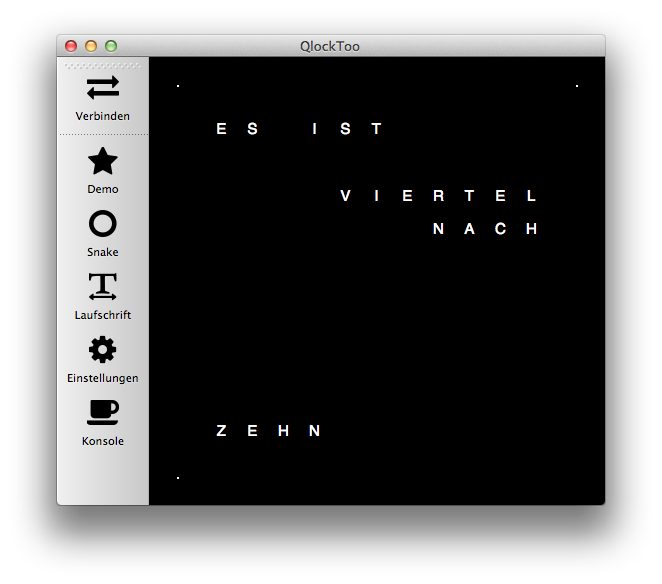
\includegraphics[width=\columnwidth]{Abbildungen/Software/Manager} % Platte gebohrt

Dieses bringt aber ein Problem mit sich. Ohne zusätzliche Streuung kann man die LED hinter dem jeweiligen Buchstaben erkennen. Eine vollständige Ausleutung ist noch nicht möglich. Um eine möglichst breite Streuung des LED-Lichtes zu erzielen, wird hinter die Buchstabenfolie eine zweite Diffusorfolie geklebt. Trotz der doppelten Folie sind die LEDs deutlich hinter den beleuchteten Buchstaben zu erkennen.

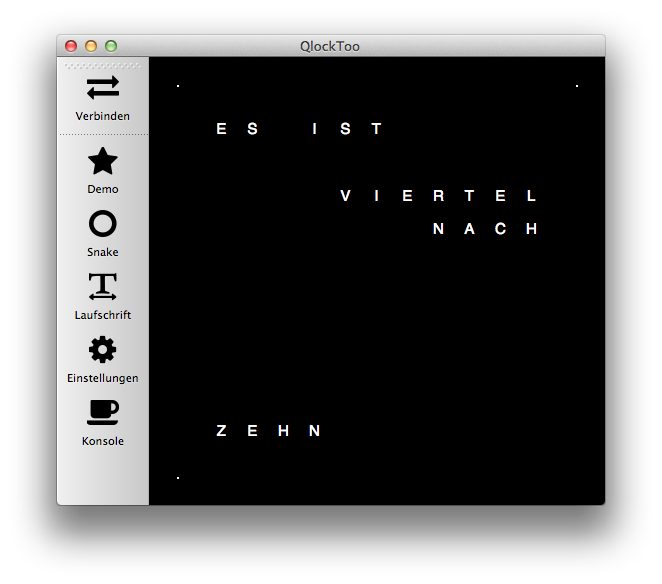
\includegraphics[width=0.9\columnwidth]{Abbildungen/Software/Manager} %Plexiglas Scheibe mit Plättchen

Um die Streuung des Lichtes zusätzlich zu erhöhen, wird ein Streuplättchen (D:~25~mm) aus transparentem Papier in die gesenkten Kegel geklebt. 

\end{multicols}

\begin{landscape}
	\begin{figure}
		\centering
		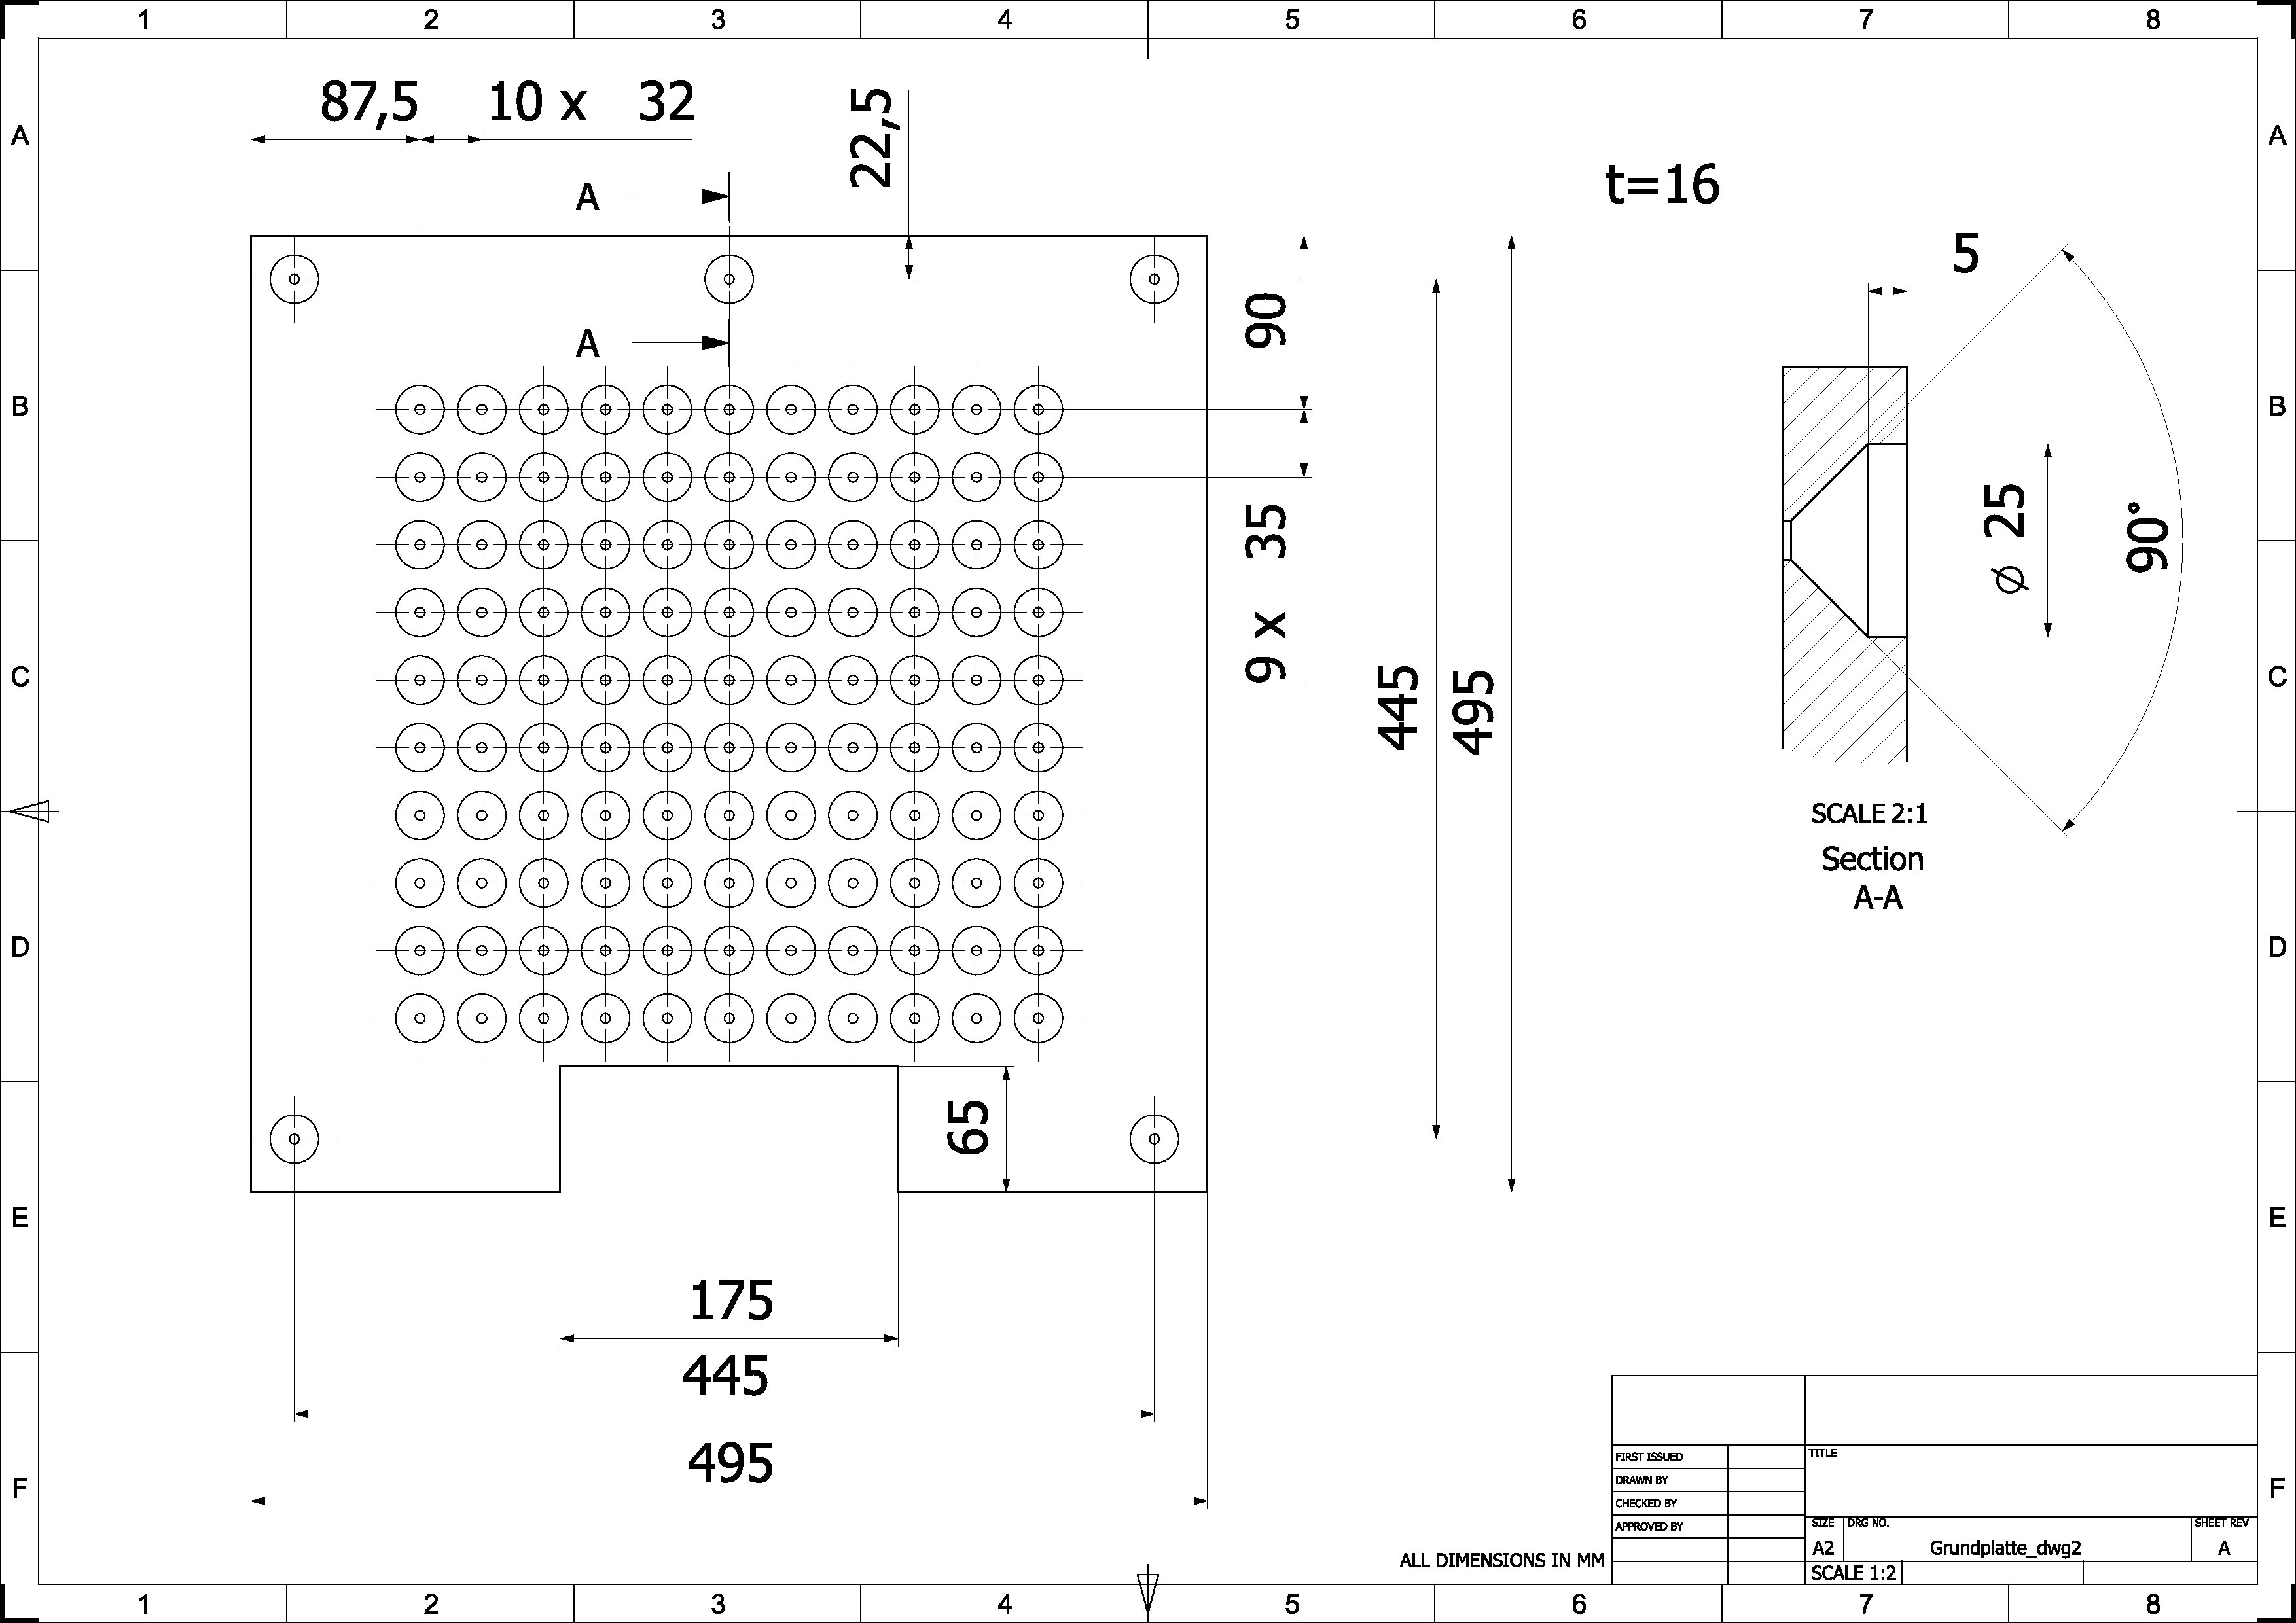
\includegraphics[width=21cm]{Abbildungen/Konstruktion/Grundplatte}
		\caption[Spanplatte]{Fertigungszeichnung Spanplatte}
		\label{fig:Spanplatte}
	\end{figure}
\end{landscape}


